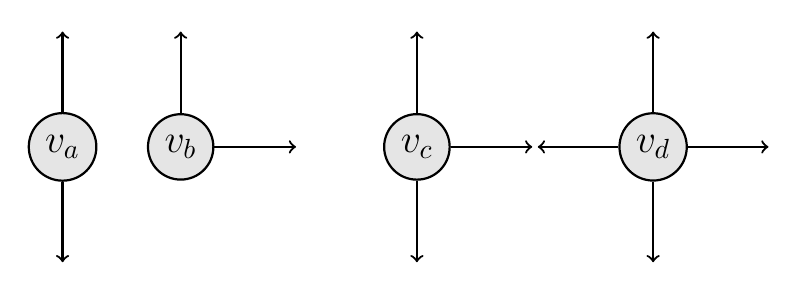
\begin{tikzpicture}[->,shorten >=1pt,auto,node distance=1.5cm,
  thick,main node/.style={circle,fill=gray!20,draw,font=\sffamily\Large\bfseries}]


  \node[main node] (2) {$v_a$};
  \coordinate[above of=2] (d5);
  \coordinate[below of=2] (d6);

  \node[main node] (3) [right of=2] {$v_b$};
  \coordinate[above of=3] (d7);
  \coordinate[right of=3] (d8);

  \node[main node] (4) [right of=d8] {$v_c$};
  \coordinate[above of=4] (d9);
  \coordinate[right of=4] (d10);
  \coordinate[below of=4] (d11);

  \node[main node] (1) [right of=d10] {$v_d$};
  \coordinate[left of=1] (d1);
  \coordinate[right of=1] (d2);
  \coordinate[above of=1] (d3);
  \coordinate[below of=1] (d4);

  \path[every node/.style={font=\sffamily\small}]
  (1)  edge [] node[above] {} (d1)
       edge [] node[above] {} (d2)
       edge [] node[above] {} (d3)
       edge [] node[above] {} (d4)

  (2)  edge [] node[above] {} (d5)
       edge [] node[above] {} (d6)

  (3)  edge [] node[above] {} (d7)
       edge [] node[above] {} (d8)

  (4)  edge [] node[above] {} (d9)
       edge [] node[above] {} (d10)
       edge [] node[above] {} (d11);
\end{tikzpicture} 
